\documentclass[usepdftitle=false,usenames,dvipsnames]{beamer}

\usetheme{focus} % see https://github.com/elauksap/focus-beamertheme
% Add option [numbering=none] to disable the footer progress bar
% Add option [numbering=fullbar] to show the footer progress bar as always full with a slide count

\usepackage{booktabs} % Required for better table rules
\usepackage{bm,times}

\usepackage{tikz}
\usetikzlibrary{decorations.pathreplacing,calc}

\usepackage{hyperref}
\hypersetup{
    pdftitle={Evolution of ice sheet geometry using Stokes dynamics}
}

\newcommand{\tikzmark}[1]{\tikz[overlay,remember picture] \node (#1) {};}

\newcommand{\eps}{\epsilon}
\newcommand{\RR}{\mathbb{R}}

\newcommand{\grad}{\nabla}
\newcommand{\Div}{\nabla\cdot}
\newcommand{\trace}{\operatorname{tr}}

\newcommand{\hbn}{\hat{\mathbf{n}}}

\newcommand{\bb}{\mathbf{b}}
\newcommand{\be}{\mathbf{e}}
\newcommand{\bbf}{\mathbf{f}}
\newcommand{\bg}{\mathbf{g}}
\newcommand{\bn}{\mathbf{n}}
\newcommand{\br}{\mathbf{r}}
\newcommand{\bu}{\mathbf{u}}
\newcommand{\bv}{\mathbf{v}}
\newcommand{\bw}{\mathbf{w}}
\newcommand{\bx}{\mathbf{x}}

\newcommand{\bF}{\mathbf{F}}
\newcommand{\bV}{\mathbf{V}}
\newcommand{\bX}{\mathbf{X}}

\newcommand{\bxi}{\bm{\xi}}

\newcommand{\bzero}{\bm{0}}

\newcommand{\rhoi}{\rho_{\text{i}}}

\newcommand{\ip}[2]{\left(#1,#2\right)}

\newcommand{\mR}{R^{\bm{\oplus}}}
\newcommand{\iR}{R^{\bullet}}

\newcommand{\pp}{{\text{p}}}
\newcommand{\qq}{{\text{q}}}
\newcommand{\rr}{{\text{r}}}

\newcommand{\bus}{\bu|_s}


\title{Evolution of \\ ice sheet geometry \\ using Stokes dynamics}

%\subtitle{Subtitle}

\author{Ed Bueler}

\titlegraphic{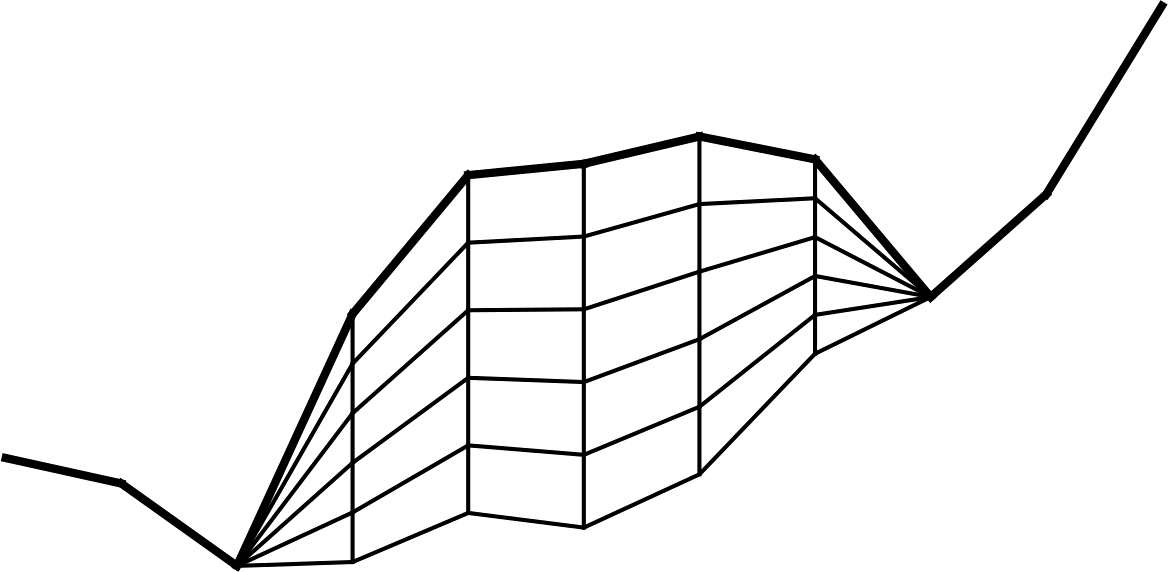
\includegraphics[width=0.7\textwidth]{figs/titleextruded.png} \\ \vspace{-8mm} 
\includegraphics[width=0.2\textwidth]{figs/uafbw.png}}

%\institute{University of Alaska Fairbanks}

\date{\phantom{foo} \bigskip \bigskip \bigskip \\ SIAM GS21}


\begin{document}

\begin{frame}
	\maketitle
\end{frame}


\begin{frame}{overview}
\Large
\begin{enumerate}
\item explain the problem I'm working on
\item mention the (current) barriers to success
\end{enumerate}

\normalsize
\vspace{10mm}
\begin{itemize}
\item work in progress
\item I am giving this talk at 4am my time
    \begin{itemize}
    \item low expectations, please
    \end{itemize}
\end{itemize}
\end{frame}


\begin{frame}{the ice geometry problem (IGP)}

\vspace{-2mm}
\begin{center}
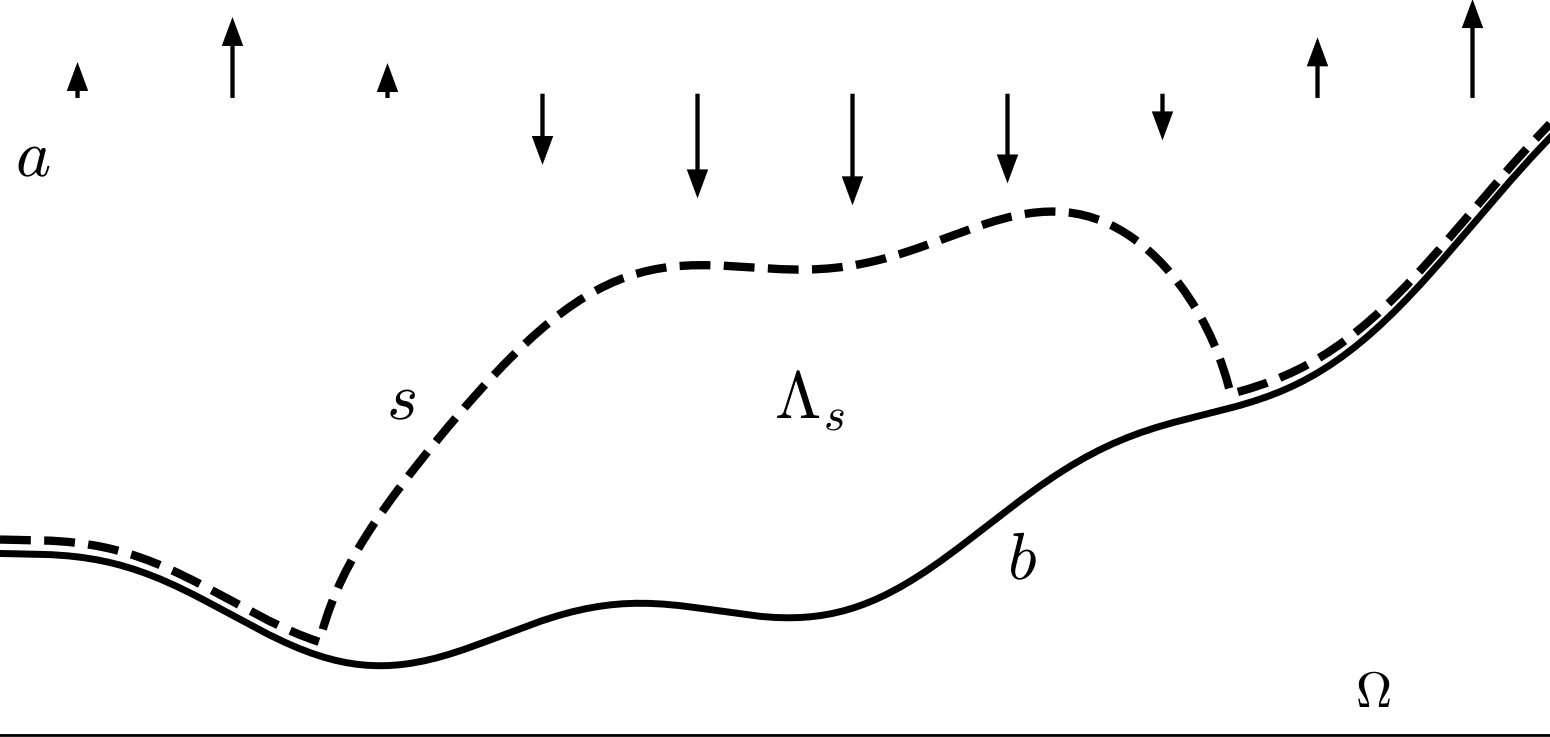
\includegraphics[width=0.7\textwidth]{figs/stokesdomain.png}
\end{center}

\vspace{-1mm}
\begin{itemize}
\item how does glacier geometry evolve in response to the climate?
\item only the simplest version (grounded, nonsliding, isothermal)
\item assume time-independent data on fixed $\Omega \subset \RR^2$:
    \begin{itemize}
    \item (net) climatic mass balance $a(x,y)$ \hfill $\gets$ \emph{$a>0$ for accumulation}
    \item bed elevation $b(x,y)$
    \end{itemize}
\item \emph{to compute}: surface elevation $s(t,x,y)$ on $\Omega$

\hspace{20.5mm} icy domain $\Lambda_s \subset \RR^3$
\end{itemize}
\end{frame}


\begin{frame}{surface kinematical equation}

\begin{itemize}
\item glaciers flow, so one must solve the surface kinematical equation (SKE) \emph{on} the ice
    $$\frac{\partial s}{\partial t} - \bu|_s \cdot \bn_s - a = 0$$

    \begin{itemize}
    \item $\bn_s = \left<-s_x,-s_y,1\right>$  \, is an upward normal to the ice surface

\vspace{4mm}
    \item where \emph{not} on the ice: $a\le 0$
    \end{itemize}
\end{itemize}

\bigskip
\begin{columns}
    \column{0.55\textwidth}
        \begin{itemize}
        \item assumed:
            \begin{itemize}
            \item $s$ well-defined (no overhangs)
            \item $s=b$ where ice is not present

                \begin{itemize}
                \item[{\color{black} $\therefore$}] $s$ is defined on all of $\Omega$
                \end{itemize}
            \end{itemize}
        \end{itemize}
    \column{0.45\textwidth}
        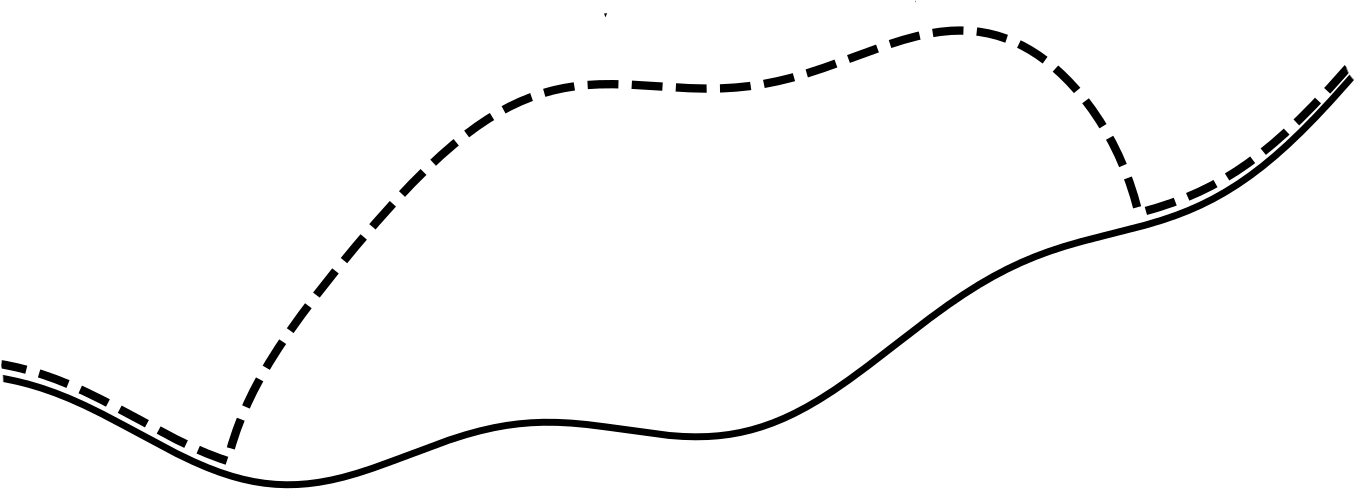
\includegraphics[width=1.0\textwidth]{figs/simpledomain.png}
\end{columns}
\end{frame}


\begin{frame}{steady IGP strong form}

\begin{itemize}
\item the \alert{steady} IGP is a \alert{nonlinear complementarity problem (NCP) for $s$}, a free-boundary problem, \alert{which is coupled to a non-Newtonian Stokes problem for $\bu,p$:}

\vspace{-5mm}

\begin{align*}
s - b &\ge 0 && \text{on $\Omega$} & \tikzmark{ncptop} \\
- \bu|_s \cdot \bn_s - a &\ge 0 && \text{''} \\
(s - b) (- \bu|_s \cdot \bn_s - a) &= 0 && \text{''} & \tikzmark{ncpbot} \\
- \nabla \cdot \left(2 \nu_\eps\, D\bu\right) + \nabla p - \rhoi \mathbf{g} &= \bzero && \text{on $\Lambda_s$} & \tikzmark{gstop} \\
\nabla \cdot \bu &= 0 && \text{''} \\
\bu &= \bzero && \text{on $\Gamma_0$ \quad (ice base)} \\
\left(2 \nu_\eps D\bu - pI\right) \bn &= \bzero && \text{on $\partial \Lambda_s \setminus \Gamma_0$} & \tikzmark{gsbot}
\end{align*}

\begin{tikzpicture}[overlay, remember picture]
\draw[decoration={brace,amplitude=0.4em},decorate,ultra thick] ([xshift=-7mm]ncptop.north east) node[right=8mm,below=3mm] {NCP} -- ([xshift=-7mm]ncpbot.east);
\end{tikzpicture}

\begin{tikzpicture}[overlay, remember picture]
\draw[decoration={brace,amplitude=0.4em},decorate,ultra thick] ([xshift=-7mm]gstop.north east) node[right=10mm,below=6mm] {Stokes} -- ([xshift=-7mm]gsbot.east);
\end{tikzpicture}

\vspace{-8mm}

    \begin{itemize}
    \item Glen-law effective viscosity with $\text{p}=(1/\text{n})+1(=4/3)$:
      $$\nu_\eps = \frac{1}{2} B_n \left(|D\bu|^2 + \eps\, D_0^2\right)^{(\pp-2)/2}$$
    \item \alert{\emph{the 3 nonlinearities}}
    \end{itemize}
\end{itemize}
\end{frame}


\begin{frame}{implicit IGP strong form}

\begin{itemize}
\item solve one step of backward Euler for $s,\bu,p$ at new time $t^\ell$
    \begin{itemize}
    \item $\frac{\partial s}{\partial t} \approx \frac{s^\ell-s^{\ell-1}}{\Delta t}$ in evolving SKE, and write $s$ for $s^\ell$
    \end{itemize}
\item at each time step, solve NCP coupled to Stokes:

\vspace{-5mm}

\begin{align*}
s - b &\ge 0 && \text{on $\Omega$} \\
\alert{s - s^{\ell-1} - \Delta t\, \bu|_s \cdot \bn_s - \Delta t\, a} &\ge 0 && \text{''} \\
(s - b) (\alert{s - s^{\ell-1} - \Delta t\, \bu|_s \cdot \bn_s - \Delta t\, a}) &= 0 && \text{''} \\
- \nabla \cdot \left(2 \nu_\eps\, D\bu\right) + \nabla p - \rhoi \mathbf{g} &= \bzero && \text{on $\Lambda_s$} \\
\nabla \cdot \bu &= 0 && \text{''} \\
\bu &= \bzero && \text{on $\Gamma_0$} \\
\left(2 \nu_\eps D\bu - pI\right) \bn &= \bzero && \text{on $\partial \Lambda_s \setminus \Gamma_0$}
\end{align*}

    \begin{itemize}
    \item \alert{very similar to steady IGP}
    \end{itemize}
\end{itemize}
\end{frame}


\begin{frame}{existing ice sheet models}

\begin{itemize}
\item almost no one is solving such a implicit or steady IGP
    \begin{itemize}
    \item except Bueler (2016), Brinkerhoff et al (2017) (\emph{shallow})
    \item and Wirbel \& Jarosch (2020) (\emph{semi-coupled, fake ice layer})
    \item none are scalable (\emph{single level})
    \end{itemize}
\item what are people doing instead, for production science?
    \begin{itemize}
    \item \alert{explicit time-stepping with $s \ge b$ enforced by truncation}
    \item usually shallow approximations, e.g.~PISM run below
    \end{itemize}

\medskip
\begin{columns}
    \column{0.7\textwidth}
        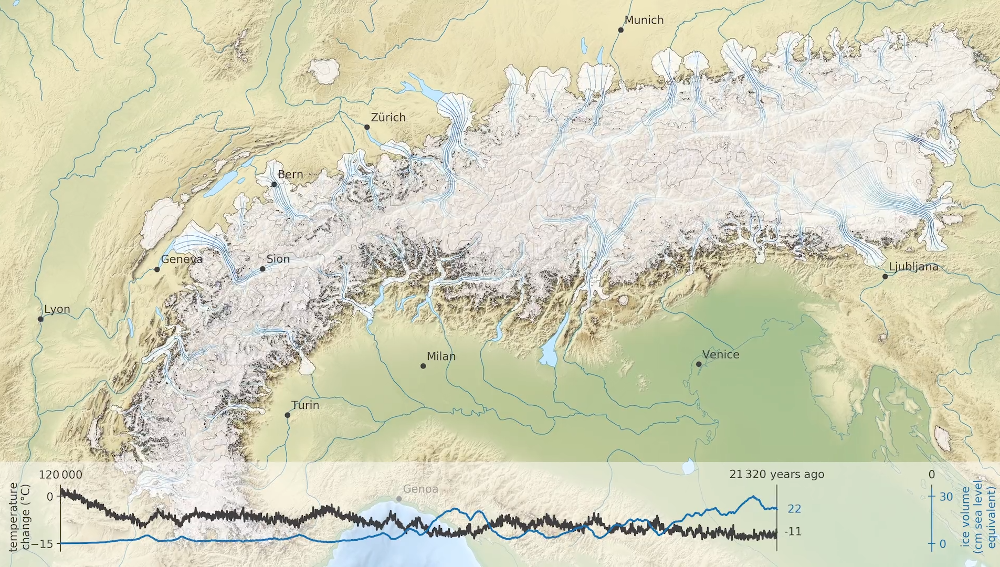
\includegraphics[width=0.8\textwidth]{figs/seguinot.png}
    \column{0.3\textwidth}
        \scriptsize \emph{by Julien Seguinot}
\end{columns}
\end{itemize}
\end{frame}


\begin{frame}{rewrite coupling as operator}

\begin{block}{ice dynamics operator}
$\Phi : s \mapsto - \bus \cdot \bn_s$

\vspace{-3mm}

\hfill 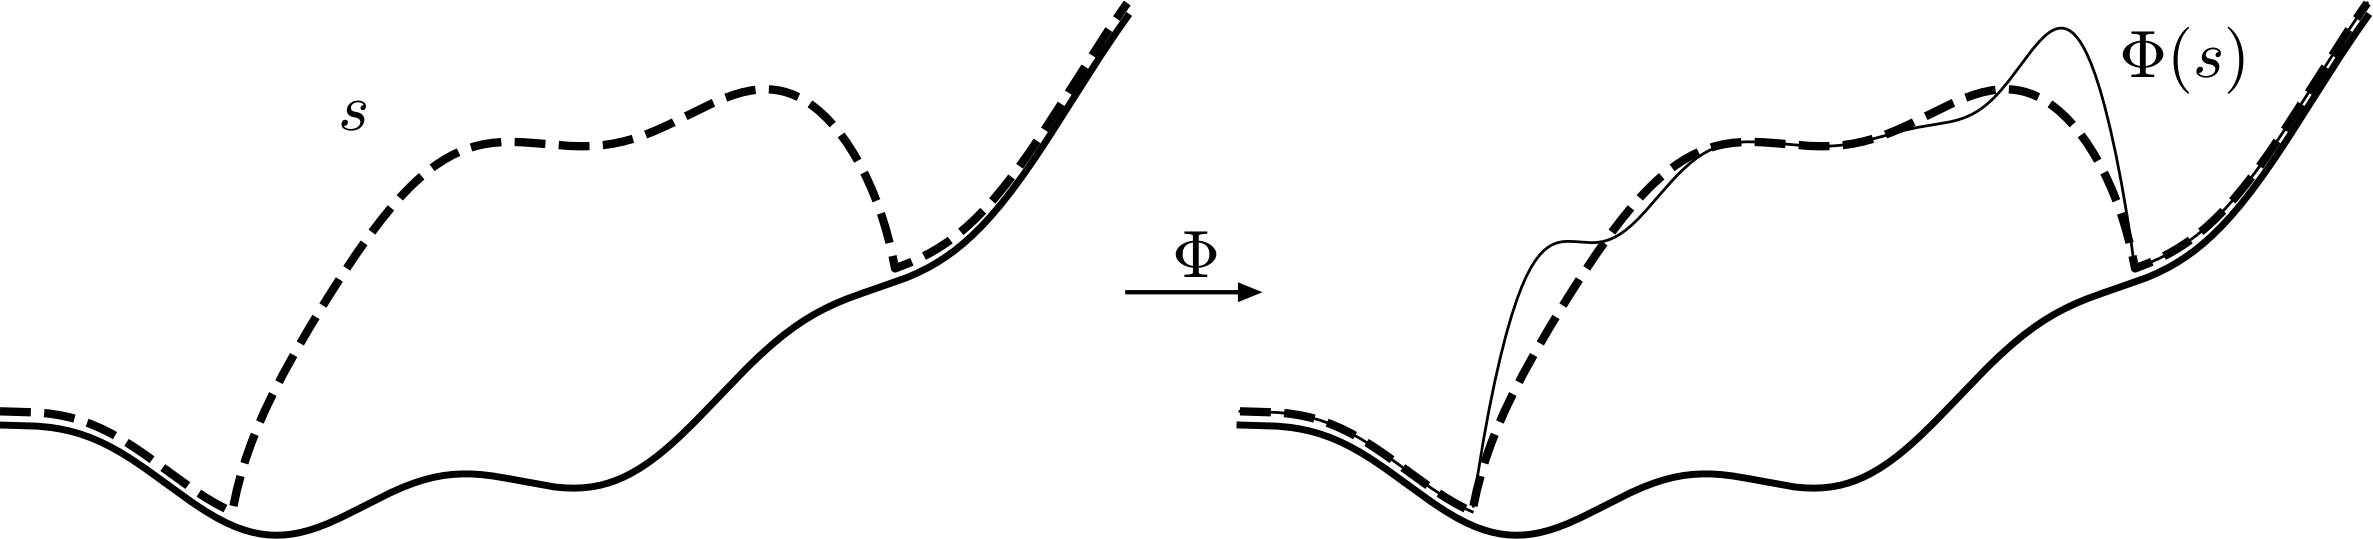
\includegraphics[width=0.7\textwidth]{figs/idoaction.png}
\end{block}

\begin{itemize}
\item to compute $\Phi(s)$: build $\Lambda_s$, solve weak-form Stokes problem
    $$F_{\Lambda_s}(\bu,p)[\bv,q] = \int_{\Lambda_s} 2 \nu_\eps D\bu : D\bv - p \Div\bv - (\Div\bu) q - \rhoi \bg \cdot \bv\,d\bx = 0,$$
extract trace $\bus$, then extend $\Phi(s) = -\bus \cdot \bn_s$ by zero to $\Omega$
\item regarding this Stokes problem (for \emph{fixed} geometry):
    \begin{itemize}
    \item well-posed over $W_0^{1,\pp}(\Lambda_s)^3 \times L^\qq(\Lambda_s)$ (Jouvet \& Rappaz 2011)
    \item optimal solver exists (Isaac et al 2015)
    \end{itemize}
\item[$\therefore$] $\phi(s)$ is well-defined if $s$ is piecewise $C^1$
    \begin{itemize}
    \item which is a regularity conjecture
    \end{itemize}
\end{itemize}

\end{frame}


\begin{frame}{IGP weak form is a variational inequality}

\begin{itemize}
\item using $\Phi$ gives a cleaner NCP over $\Omega$ for the steady IGP:
\begin{align*}
s - b &\ge 0 \\
\Phi(s) - a &\ge 0 \\
(s - b) (\Phi(s) - a) &= 0
\end{align*}

    \begin{itemize}
    \item recall NCP (strong form) $\leftrightarrow$ VI (weak form)
    \end{itemize}

\begin{block}{steady IGP weak form}
find admissible $s \in \mathcal{K} = \{r \ge b\} \subset W^{1,\qq}(\Omega)$ so that
    $$\ip{\Phi(s)-a}{r-s} \ge 0 \qquad \text{ for all } r \in \mathcal{K}$$
\end{block}

\item well-posedness is almost completely open
    \begin{itemize}
    \item existence holds for SIA version (Jouvet \& Bueler, 2012)
    \end{itemize}

\end{itemize}
\end{frame}


\begin{frame}{what kind of beast is $\Phi$?}

\begin{center}
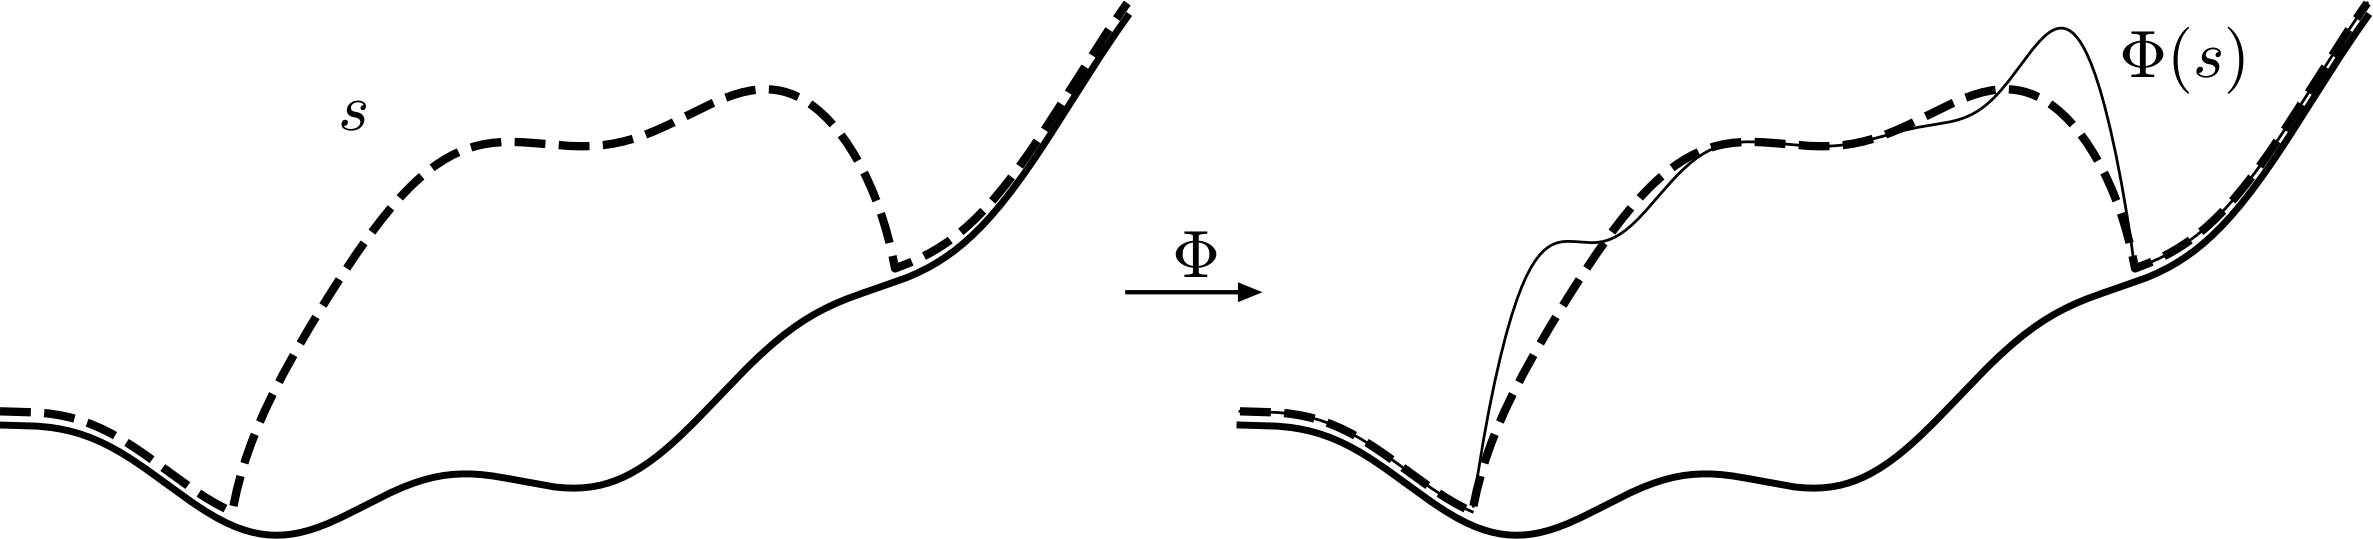
\includegraphics[width=0.7\textwidth]{figs/idoaction.png} \hfill 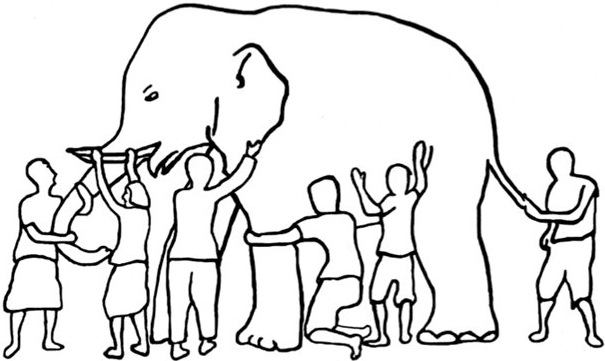
\includegraphics[width=0.2\textwidth]{figs/elephant.png}
\end{center}

\begin{itemize}
\small
\item $\Phi : \mathcal{K} \subset W^{1,\qq}(\Omega) \to W^{-1,\pp}(\Omega)$ where $\qq=4$ and $\pp=4/3$
\item the Stokes stress balance is nonlocal
    \begin{itemize}
    \item $\Phi$ is integral operator (\emph{convolve with Stokeslets})
    \item $\Phi$ is short range (\emph{dense but concentrated near the diagonal})
    \end{itemize}
\item $\Phi \approx \Phi_{\text{SIA}}$ for shallow glaciers, a differential operator:
    $$\Phi_{\text{SIA}}(s) = - \frac{\gamma}{\qq} (s-b)^{\qq} |\grad_2 s|^{\qq} - \grad_2 \cdot\left[\frac{\gamma}{\qq+1} (s-b)^{\qq+1} |\grad_2 s|^{\qq-2} \grad_2 s\right]$$

    \begin{itemize}
    \item $\Phi$ is elliptic ``in the large''
    \item $\Phi$ is degenerate at the ice margin
    \end{itemize}
\item yet common to say
    \begin{itemize}
    \item $\Phi$ is advective because SKE is write-able as a transport equation for thickness: $H_t + \overline{\bu}\, \grad H = a$
    \end{itemize}
\end{itemize}
\end{frame}


\begin{frame}{goal: robust and optimal IGP solver}

\begin{block}{numerical problem}
given triangulation $\mathcal{T}$ of $\Omega$ and $P_1$ space $\mathcal{V}^h \subset W^{1,\qq}(\Omega)$, and convex set $\mathcal{K}^h = \{r^h \ge b^h\} \subset \mathcal{V}^h$, solve VI for $s^h \in \mathcal{K}^h$:

$$\ip{\Phi^h(s^h) - a}{r^h - s^h} \ge 0 \qquad \text{for all $r^h \in \mathcal{K}^h$}$$
\end{block}

\begin{itemize}
\item[]
    \begin{itemize}
    \item $P_1$ because of low regularity at free boundary
    \item evaluate $\Phi^h(s^h)=-\bu|_{s^h}\cdot\bn_{s^h}$ by solving Stokes problem $F_{\Lambda_{s^h}}(\bu^h,p^h)=0$
    \end{itemize}
\item seeking a solver which is:
    \begin{itemize}
    \item \alert{robust}
    \item \alert{near optimal} $O(m^{1+\eps})$ work over $m$ degrees of freedom in $\mathcal{V}^h$
        \begin{itemize}
        \item[{\color{black} $\circ$}] requires multigrid \dots more below
        \end{itemize}
    \item \emph{these are aspirations}
    \end{itemize}
\end{itemize}
\end{frame}


\begin{frame}{smoothness and multilevel methods}

\begin{columns}
\column{0.35\textwidth}
    \begin{itemize}
    \small
    \item which solution variable?
        \begin{itemize}
        \item surface elevation $s$?
        \item thickness $H$?
        \end{itemize}
    \end{itemize}
\column{0.65\textwidth}
    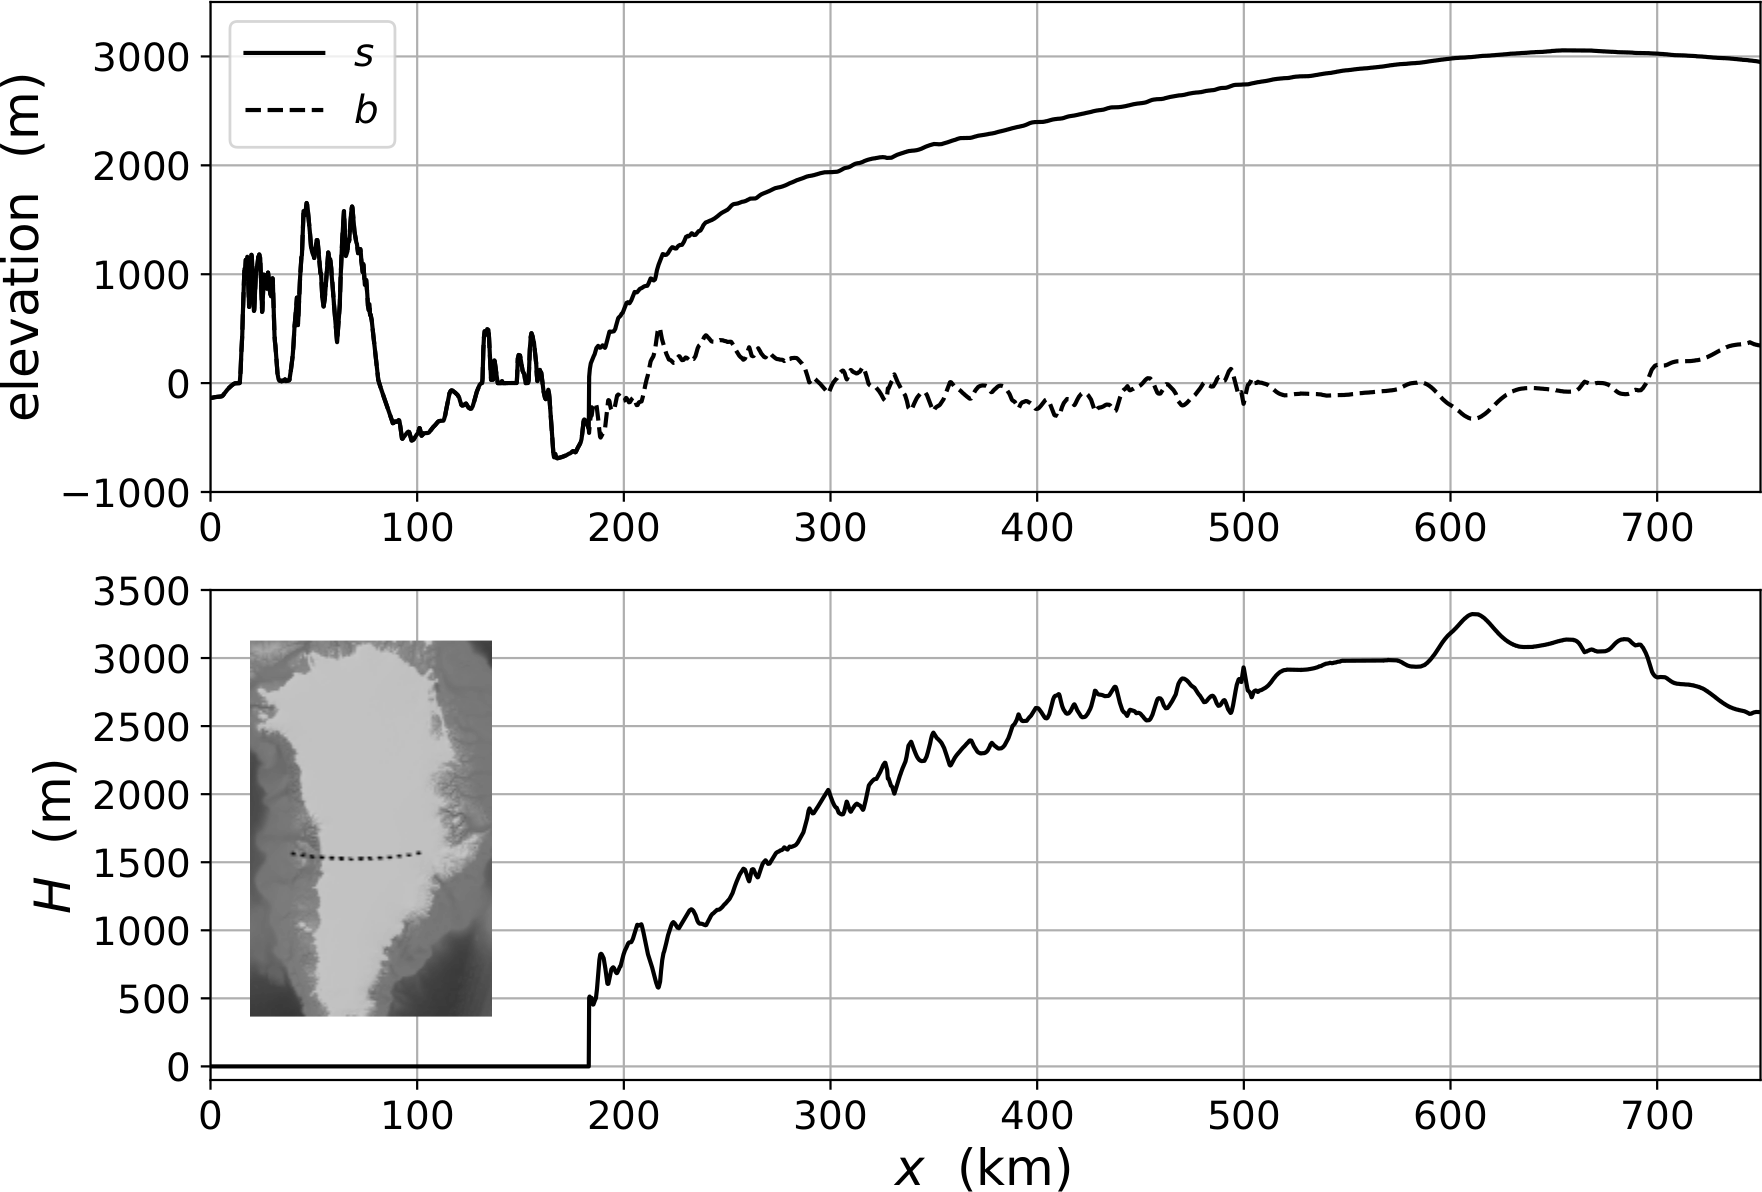
\includegraphics[width=\textwidth]{figs/giscross.png}
\end{columns}

\bigskip
\begin{itemize}
\item \alert{smoothness suggests $s$ is better for multigrid}
    \begin{itemize}
    \item but \emph{do not} put ``fake ice'' where $s=b$; only solve for ice velocity where there is ice!
    \end{itemize}
\end{itemize}
\end{frame}


\begin{frame}{multilevel constraint decomposition (MCD)}

\begin{block}{strategy}
decompose $\mathcal{K}^h$ using mesh hierarchy and then apply V-cycles
\end{block}

\bigskip
\begin{columns}
\column{0.52\textwidth}
\begin{itemize}
\item mesh levels over $\Omega$:

$\mathcal{T}^0 \text{ (coarse) to } \mathcal{T}^J$
\item given fine-level iterate $s^J$
\item \emph{defect constraint} $\chi^J = b^J - s^J$
\item \emph{monotone restriction} $R^\oplus$

\item defect constraints on levels:

$\chi^j = R^\oplus \chi^{j+1}$
\item admissible perturbations:

$z^j \ge \chi^j \iff s^j + z^j \ge b^j$
\end{itemize}
\column{0.48\textwidth}
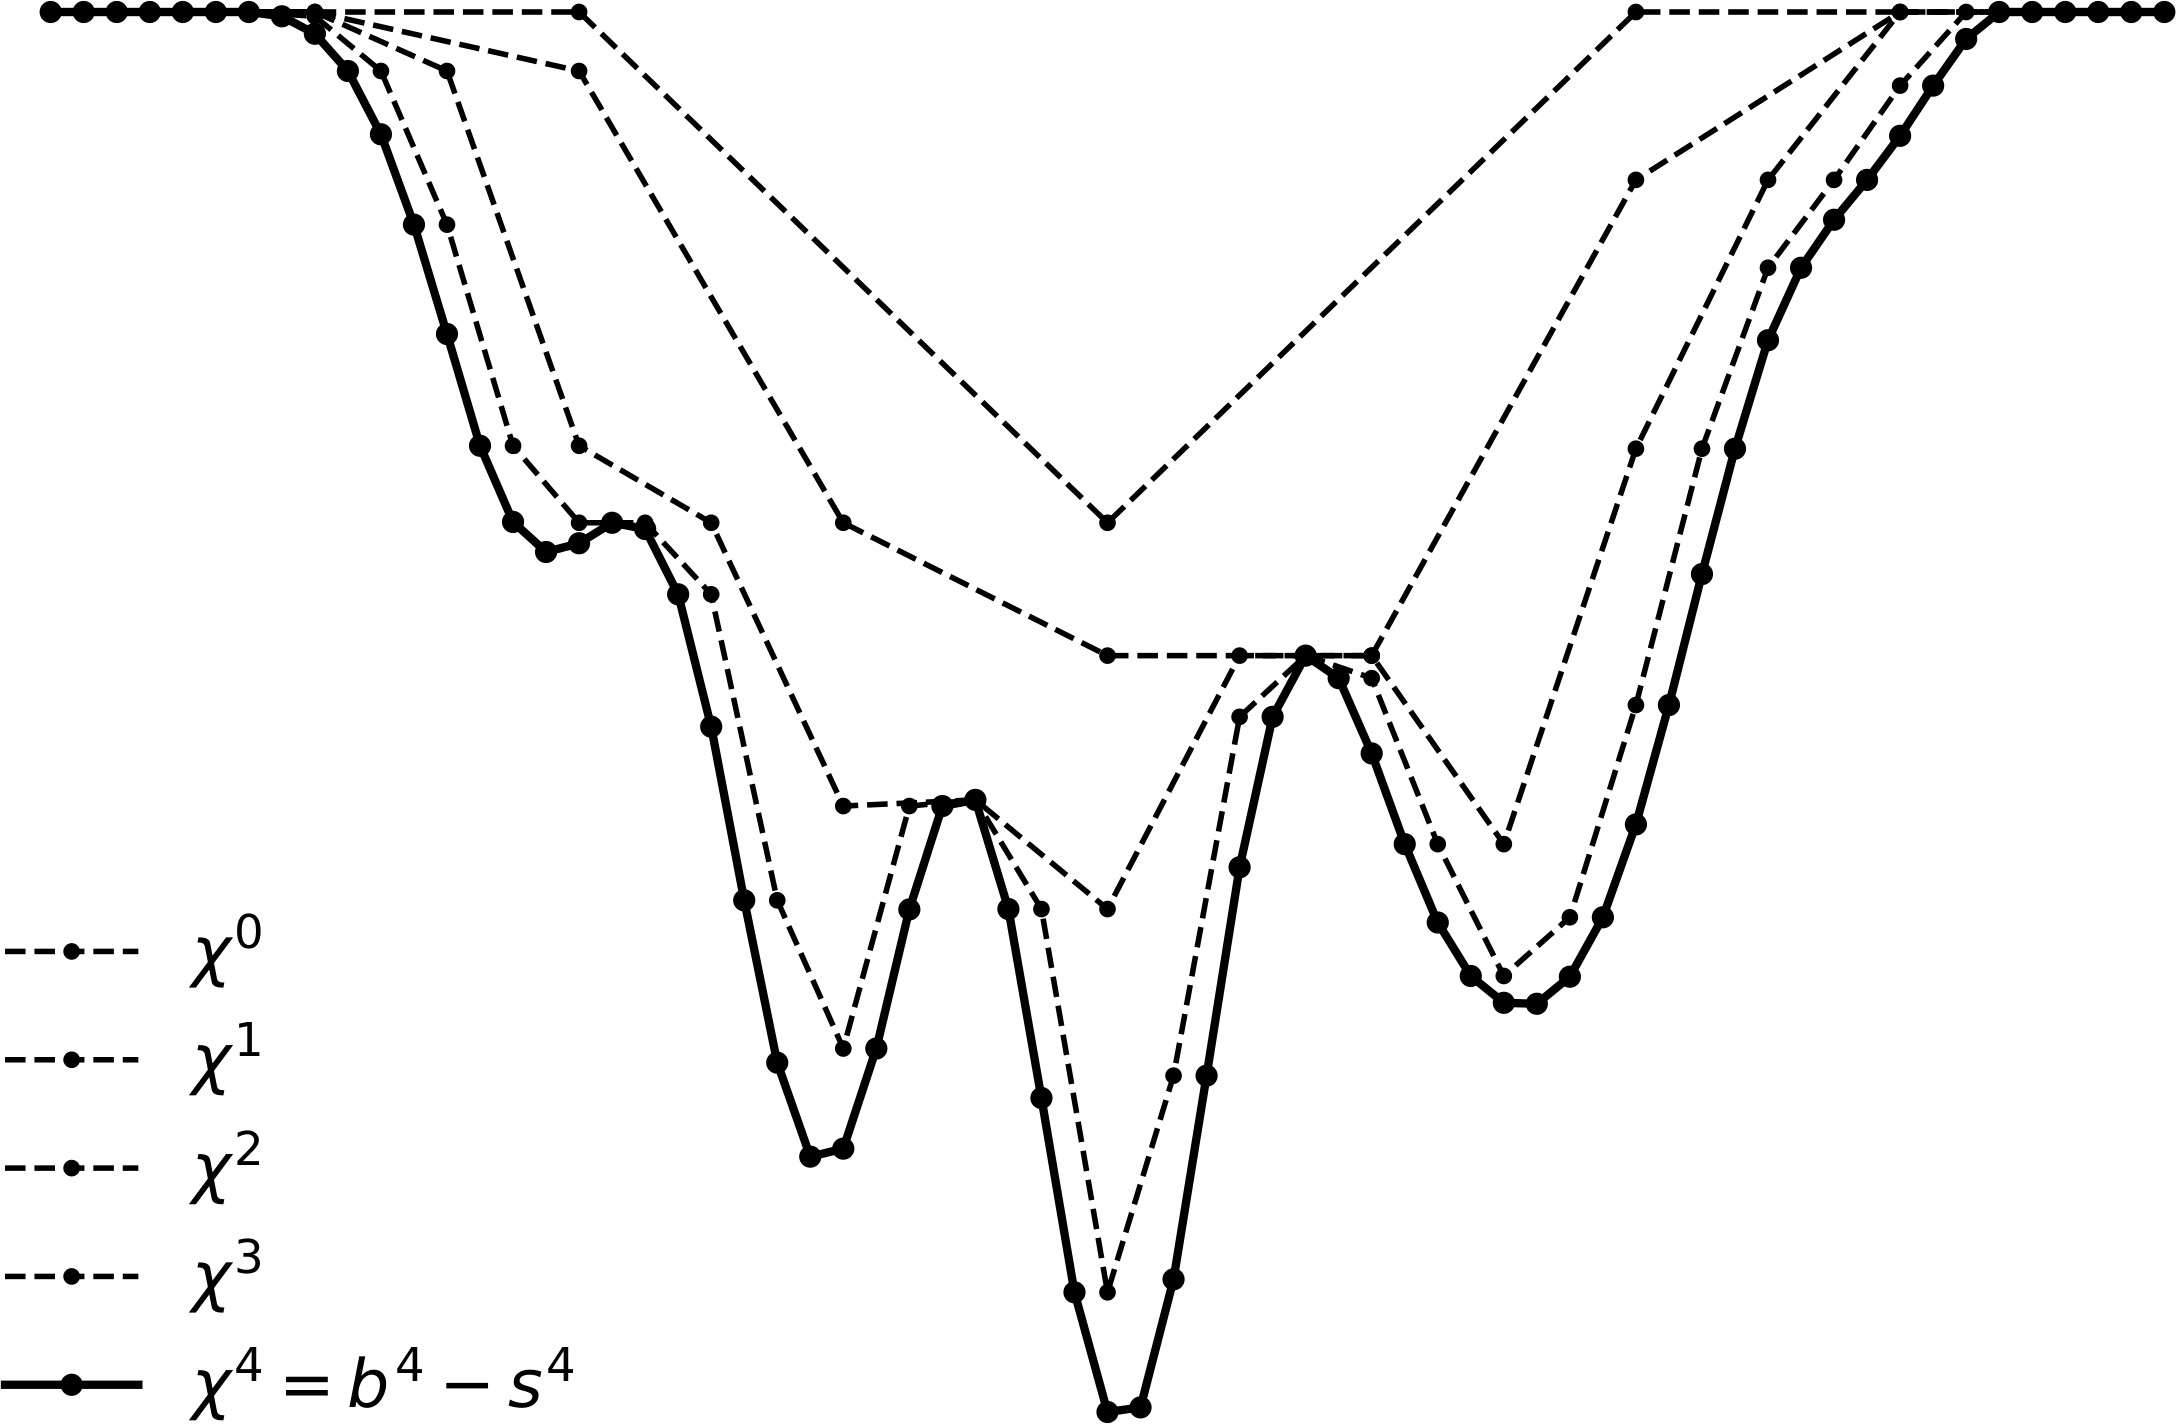
\includegraphics[width=1.05\textwidth]{figs/decompclassical.png}
\end{columns}
\end{frame}


\begin{frame}{multilevel constraint decomposition (MCD)}

\begin{itemize}
\item in V-cycle, on each level solve a VI:
    $$\ip{\Phi^j(s^j + z^j) - a^j}{v^j - z^j} \ge 0 \quad \text{ for all $v^j \ge \chi^j$}$$

\item this strategy gives an $O(m\log m)$ solver for the Laplacian obstacle problem (Tai, 2003)
    \begin{itemize}
    \item \alert{a multilevel VI strategy is the only hope for (near) optimality}
    \end{itemize}
\item for IGP:
    \begin{itemize}
    \item for nonlinear VI, need additional FAS strategy {\Large\strut} {\color{ForestGreen} \, {\Large $\checkmark$}}
    \item \dots but each residual is nonlocal and expensive
    \end{itemize}
\end{itemize}
\end{frame}


\begin{frame}{Stokes on a Firedrake extruded mesh}

\begin{center}
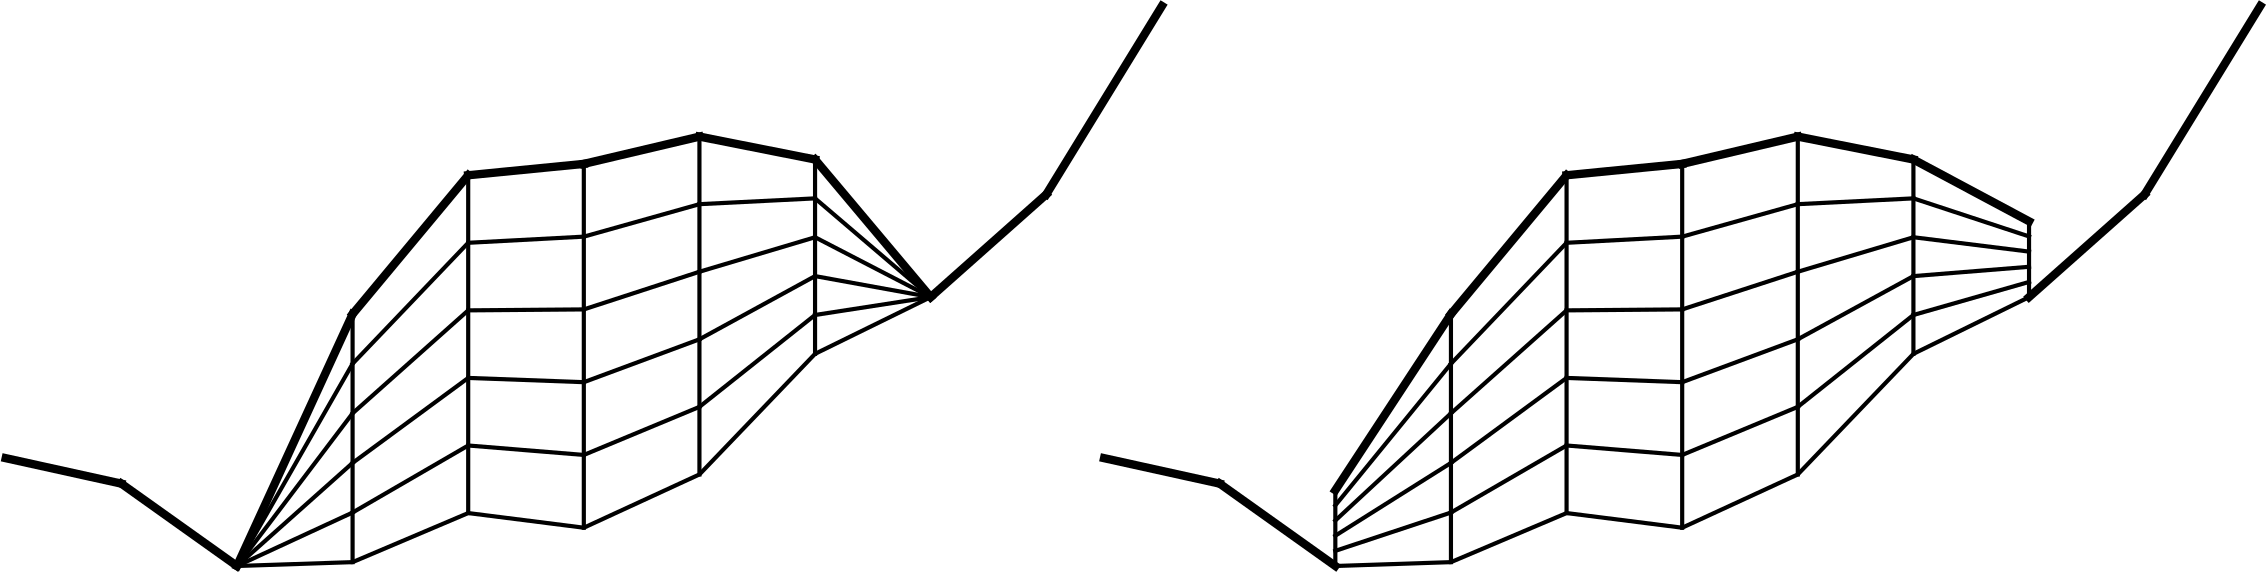
\includegraphics[width=0.8\textwidth]{figs/extruded.png}
\end{center}

\begin{columns}
\column{0.77\textwidth}
\begin{itemize}
\item V-cycle based on mesh hierarchy $\{\mathcal{T}^j\}$ over $\Omega$
\item to evaluate the residual $\Phi(s^j) - a^j$ in the VI:
    \begin{itemize}
    \item extrude base mesh $\mathcal{T}^j$ to current geometry $s^j$
        \begin{itemize}
        \item[{\color{black} $\circ$}] with or without small cliffs
        \end{itemize}
    \item no extrusion where ice free
        \begin{itemize}
        \item[{\color{black} $\circ$}] thanks to Lawrence Mitchell for this capability
        \end{itemize}
    \item solve Stokes problem $F_{\Lambda_{s^j}}(\bu^j,p^j)=0$
    \item compute $\Phi(s^j) = - \bu^j|_{s^j} \cdot \bn_{s^j}$ and subtract $a^j$
    \end{itemize}
\end{itemize}
\column{0.23\textwidth}
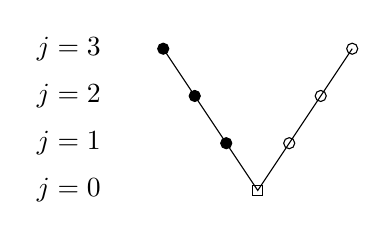
\begin{tikzpicture}[scale=0.8]
  \pgfmathsetmacro\hstep{0.5}
  \pgfmathsetmacro\vstep{0.75}
  \pgfmathsetmacro\ceps{0.08}   % size of square for coarse grid

% grid labels at left
  \node at (-2,3*\vstep) {$j=3$};
  \node at (-2,2*\vstep) {$j=2$};
  \node at (-2,\vstep) {$j=1$};
  \node at (-2,0.0) {$j=0$};

% V-cycle
  \draw[black,thin] (-\hstep,3*\vstep) -- (0.0,2*\vstep) -- (\hstep,\vstep) --  (2*\hstep,0.0)
                    -- (3*\hstep,\vstep) -- (4*\hstep,2*\vstep) -- (5*\hstep,3*\vstep);
  \filldraw (-\hstep,3*\vstep) circle (2.5pt);
  \filldraw (0.0,2*\vstep) circle (2.5pt);
  \filldraw (\hstep,\vstep) circle (2.5pt);
  \draw     (2*\hstep-\ceps,-\ceps) rectangle (2*\hstep+\ceps,+\ceps);
  \draw     (3*\hstep,\vstep) circle (2.5pt);
  \draw     (4*\hstep,2*\vstep) circle (2.5pt);
  \draw     (5*\hstep,3*\vstep) circle (2.5pt);
\end{tikzpicture}

\end{columns}
\end{frame}


\begin{frame}{smoother options}

\begin{itemize}
\item now all the evil is in the smoother
\item smoother options from weaker to stronger:
    \begin{itemize}
    \item nonlinear Richardson?
    \item exploit SIA analogy?
        \begin{itemize}
        \item[{\color{black} $\circ$}] pointwise smoothers work for SIA
        \end{itemize}
    \item nonlinear pointwise smoothers (GS, Jacobi)?
        \begin{itemize}
        \item[{\color{black} $\circ$}] \alert{GS extremely expensive because residual nonlocal}
        \item[{\color{black} $\circ$}] seem to fail
        \end{itemize}
    %\item nonlinear and nonlocal \texttt{PCPatch} smoothers?
    %    \begin{itemize}
    %    \item[{\color{black} $\circ$}] what does this even mean?
    %    \end{itemize}
    \item reduced-space Newton using banded Jacobian approximation?
        \begin{itemize}
        \item[{\color{black} $\circ$}] finite-difference Jacobian entries using pseudo-coloring
        \end{itemize}
    \end{itemize}
\end{itemize}
\end{frame}


\begin{frame}{status report}

\begin{itemize}
\item \alert{nothing works well so far}
\end{itemize}
\end{frame}


\begin{frame}{conclusion}

\begin{itemize}
\item \emph{GOAL 1}:\, no shallow approximations in flow physics
    \begin{itemize}
    \item[{\Large \color{ForestGreen} $\checkmark$}] Stokes solver working in Firedrake on extruded mesh
    \item[{\Large \color{ForestGreen} $\checkmark$}] solver choices by (Isaac et al, 2015) putatively optimal
    \end{itemize}
\item \emph{GOAL 2}:\, beat explicit time-stepping
    \begin{itemize}
    \item[{\Large \color{ForestGreen} $\checkmark$}] observe that problem is
        \begin{itemize}
        \item[{\color{black} $\circ$}] constrained (nonlinear VI on $\mathcal{K} = \{s\ge b\}$)
        \item[{\color{black} $\circ$}] diffusive in the large (Stokes $\approx$ SIA)
        \item[{\color{black} $\circ$}] nonlocal (Stokes)
        \end{itemize}
    \item[{\Large \color{ForestGreen} $\checkmark$}] MCD FAS path to optimality for solving the VI
    \item[{\Large \alert{:-(}}] \alert{stuck on finding a robust, efficient smoother}
    \end{itemize}
\end{itemize}

\begin{block}{ultimate goal}
for better science, enable long-time (paleo) simulations without shallow approximations
\end{block}

\emph{thanks for your attention \dots questions?}
\end{frame}

%\begin{block}{Block}
%\begin{alertblock}{Alert block}
%	\pause % Automatically creates a new "page" split between the above and above + below
%	\begin{exampleblock}{Example block}


%\begin{frame}{Columns}
%	\begin{columns}
%		\column{0.5\textwidth}
%			This text
%		\column{0.5\textwidth}
%			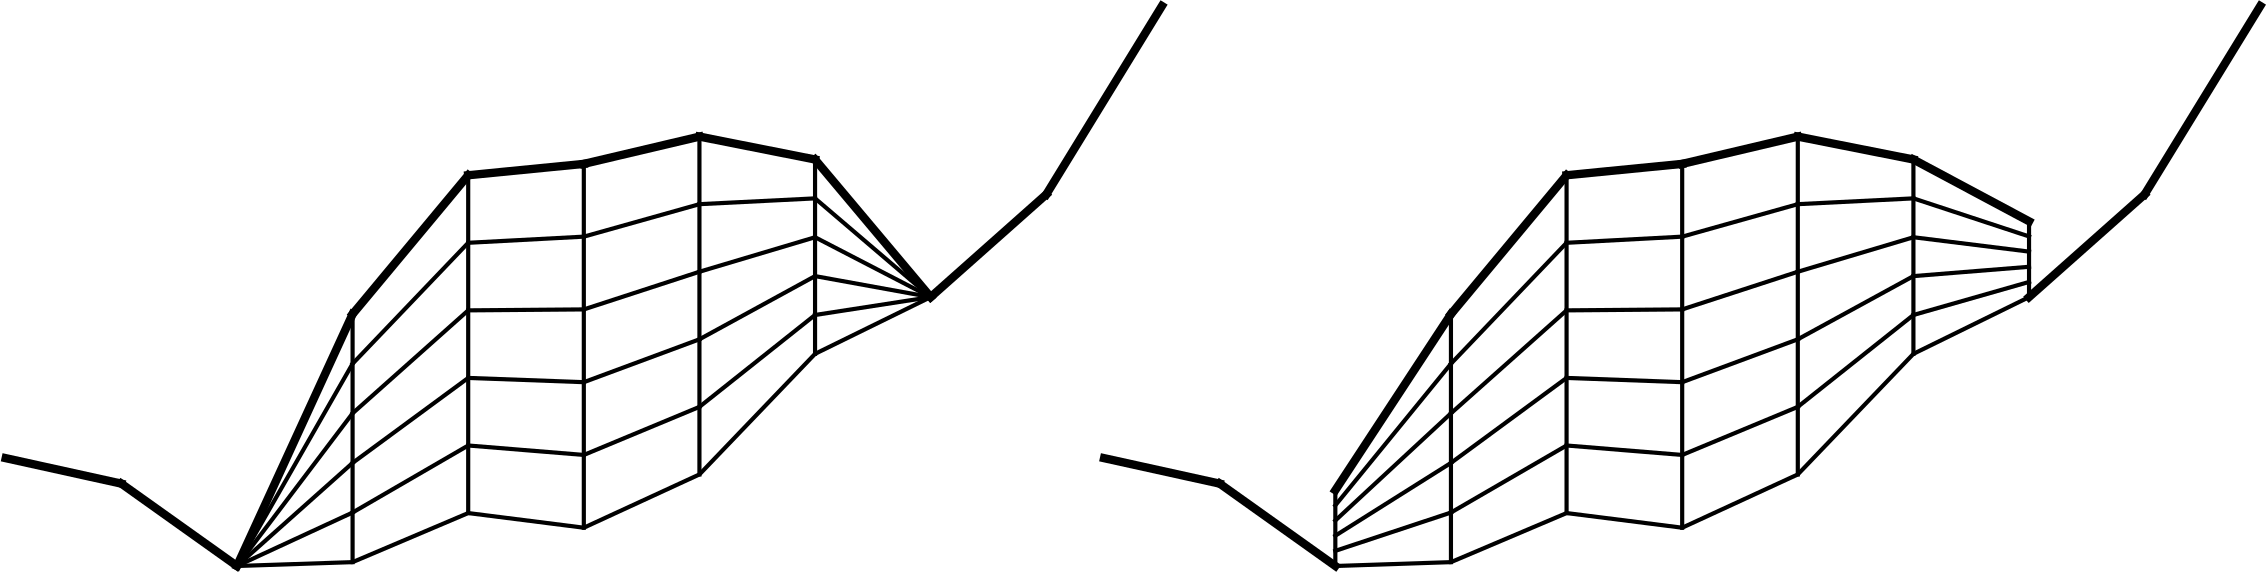
\includegraphics[width=\linewidth]{figs/extruded.png}
%	\end{columns}
%\end{frame}


\appendix

\begin{frame}{Some references 1}
%\nocite{*}
%\bibliography{../paper/msg.bib}
%\bibliographystyle{plain}

\begin{thebibliography}{1}
\bibitem{Brinkerhoffetal2017}
D.~Brinkerhoff, M.~Truffer, and A.~Aschwanden. \textbf{Sediment transport drives tidewater glacier periodicity.} {\em Nature Communications}, 8(1):1--8, 2017.

\bibitem{Bueler2016}
E.~Bueler. \textbf{Stable finite volume element schemes for the shallow-ice approximation.} {\em J. Glaciol.}, 62 (232):230--242, 2016.

\bibitem{IsaacStadlerGhattas2015}
T.~Isaac, G.~Stadler, and O.~Ghattas.  \textbf{Solution of nonlinear Stokes equations \dots with application to ice sheet dynamics.} {\em SIAM J. Sci. Comput.}, 37(6):B804--B833, 2015.

\bibitem{JouvetBueler2012}
G.~Jouvet and E.~Bueler. \textbf{Steady, shallow ice sheets as obstacle problems: well-posedness and finite element approximation.} {\em SIAM J. Appl. Math.}, 72(4):1292--1314, 2012.

\bibitem{JouvetRappaz2011}
G.~Jouvet and J.~Rappaz. \textbf{Analysis and finite element approximation of a nonlinear stationary {S}tokes problem arising in glaciology.} {\em Advances in Numerical Analysis}, 2011.
\end{thebibliography}
\end{frame}


\begin{frame}{Some references 2}
\begin{thebibliography}{1}
\bibitem{Tai2003}
X.-C. Tai. \textbf{Rate of convergence for some constraint decomposition methods for nonlinear variational inequalities.} {\em Numer. Math.}, 93(4):755--786, 2003.

\bibitem{WirbelJarosch2020}
A.~Wirbel and A.~H. Jarosch. \textbf{Inequality-constrained free-surface evolution in a full {S}tokes ice flow model \dots} {\em Geosci. Model Dev.}, 13(12):6425--6445, 2020.
\end{thebibliography}
\end{frame}


\begin{frame}{extra}

NCP is a barrier to exact numerical mass conservation\footnote{E.~Bueler. \textbf{Conservation laws for free-boundary fluid layers.} \em{SIAM J.~Appl.~Math.}, to appear.}
\end{frame}
\end{document}
